\documentclass[UTF8]{article}
\usepackage{cite}
\usepackage[unicode,pdftex]{hyperref}
\usepackage{enumerate}
% \usepackage{geometry}
\usepackage{setspace}
\usepackage{pslatex} 
\usepackage{fancyhdr}
\usepackage{float}
\usepackage{amsmath}
\usepackage{titling}
\usepackage{indentfirst}
\usepackage{graphicx}
\usepackage{wrapfig}
\usepackage{amsmath}
\usepackage{xstring}
\usepackage{multirow}
\usepackage{amsmath}
\usepackage{verbatim}
\usepackage{multirow}
\usepackage{array}
\usepackage{diagbox}[2011/11/22]
\usepackage{mathrsfs}
\usepackage{amsfonts}
\usepackage{mathtools}
\usepackage{multirow}
\usepackage{xcolor}
\usepackage{amssymb}
\usepackage{listings}
\usepackage{color}
\usepackage{tikz}
\usetikzlibrary{fit, calc}
\pagestyle{empty} 



% \geometry{left=2.5cm, right=2.5cm, top=1.4cm, bottom=2.4cm}
\usepackage[a4paper,top=3cm,bottom=2cm,left=3cm,right=3cm,marginparwidth=1in, margin=1in]{geometry}
% \usepackage[margin=1in]{geometry}
\title{Assignment 2 Report}
\author{Chenqiu Zhao(zhao.chenqiu@ualberta.ca)}
\date{}


\definecolor{dkgreen}{rgb}{0,0.6,0}
\definecolor{gray}{rgb}{0.5,0.5,0.5}
\definecolor{mauve}{rgb}{0.58,0,0.82}

\lstset{frame=tb,
  language=Python,
  aboveskip=3mm,
  belowskip=3mm,
  showstringspaces=false,
  columns=flexible,
  basicstyle={\small\ttfamily},
  numbers=none,
  numberstyle=\tiny\color{gray},
  keywordstyle=\color{blue},
  commentstyle=\color{dkgreen},
  stringstyle=\color{mauve},
  breaklines=true,
  breakatwhitespace=true,
  tabsize=3
}

\definecolor{codegreen}{rgb}{0,0.6,0}
\definecolor{codegray}{rgb}{0.5,0.5,0.5}
\definecolor{codepurple}{rgb}{0.58,0,0.82}
\definecolor{backcolour}{rgb}{1,1,1}
 
\lstdefinestyle{mystyle}{
    backgroundcolor=\color{backcolour},   
    commentstyle=\color{codegreen},
    keywordstyle=\color{magenta},
    numberstyle=\tiny\color{codegray},
    stringstyle=\color{codepurple},
    basicstyle=\ttfamily\footnotesize,
    breakatwhitespace=false,         
    breaklines=true,                 
    captionpos=b,                    
    keepspaces=true,                 
    numbers=left,                    
    numbersep=5pt,                  
    showspaces=false,                
    showstringspaces=false,
    showtabs=false,                  
    tabsize=2,
    escapeinside=``
}
 
\lstset{style=mystyle}

\newcommand{\reffig}[1]{Fig. \ref{#1}}
\newcommand{\refsec}[1]{Section \ref{#1}}
% \newcommand{\refeq}[1]{Eq. \ref{#1}}
\newcommand{\reftab}[1]{Table \ref{#1}}
\newcommand{\tabincell}[2]{\begin{tabular}{@{}#1@{}}#2\end{tabular}}
\newcommand{\refequ}[1]{Eqn. \ref{#1}}


\renewcommand{\tabincell}[2]{\begin{tabular}{@{}#1@{}}#2\end{tabular}}


\fancyhead{}
\lhead{\scriptsize Chenqiu Zhao}
\rhead{\scriptsize research Proposal}

\renewcommand{\headrulewidth}{0pt}
\renewcommand{\normalsize}{\fontsize{12pt}{\baselineskip}\selectfont}


\newcommand{\chronoperiode}[7]{
  \pgfmathsetmacro{\first}{(#2 - 2018)*12 + #3 - .9} % beginig of the peropd
  \pgfmathsetmacro{\last}{(#4 - 2018)*12 + #5 - 1.1} % end of the period
  \pgfmathsetmacro{\middle}{(\first+\last)/2} % position of the country name
  \fill[#7] (\first,#6-1) rectangle (\last,#6) (\middle,#6-.5) node[white, font=\sf]{#1};
}

\definecolor{level1}{RGB}{200,10,20}
\definecolor{brightube}{rgb}{0.82, 0.62, 0.91}
\definecolor{fuchsia}{rgb}{1.0, 0.0, 1.0}
\definecolor{heliotrope}{rgb}{0.87, 0.45, 1.0}



\begin{document}
\maketitle
%\vspace{-90pt}

%\section*{Abstract}
%\label{sec_abs}
In this assignment, three python source files are proposed corresponding to question 1 , question 2 and question 3 respectively.
The mathematical proof of question 4 is proposed in the last section.


\section*{Question 1}
\label{sec_q}
To replace the sum of squared difference (SSD) by mutual information neural estimation (MINE), two key functions and a key class are implemented,
please check ``\textbf{question1.py}'' for more details.
Mine network is implemented in a class, in which three linear layers with the size of $2 \times 10$, $10 \times 10$ and $10 \times 1$ are contained.
The source code is shown as below:
\begin{lstlisting}
class Mine(nn.Module):
    def __init__(self, input_size=2, hidden_size=100):
        super().__init__()
        self.fc1 = nn.Linear(input_size, hidden_size)
        self.fc2 = nn.Linear(hidden_size, hidden_size)
        self.fc3 = nn.Linear(hidden_size, 1)
        nn.init.normal_(self.fc1.weight,std=0.02)
        nn.init.constant_(self.fc1.bias, 0)
        nn.init.normal_(self.fc2.weight,std=0.02)
        nn.init.constant_(self.fc2.bias, 0)
        nn.init.normal_(self.fc3.weight,std=0.02)
        nn.init.constant_(self.fc3.bias, 0)

    def forward(self, input):
        output = F.elu(self.fc1(input))
        output = F.elu(self.fc2(output))
        output = self.fc3(output)
        return output
\end{lstlisting}

Since there is a sampling procedure in the Mine loss, the function \textbf{sample\_batch} is implemented as below:
\begin{lstlisting}
def sample_batch(data, batch_size=100, sample_mode='joint'):
    if sample_mode == 'joint':
        index = np.random.choice(range(data.shape[0]), size=batch_size, replace=False)
        batch = data[index]
    else:
        joint_index = np.random.choice(range(data.shape[0]), size=batch_size, replace=False)
        marginal_index = np.random.choice(range(data.shape[0]), size=batch_size, replace=False)

        batch = torch.cat((data[joint_index][:,0].reshape(-1,1),
                                         data[marginal_index][:,1].reshape(-1,1)), 1)
    return batch
\end{lstlisting}

Finally, the function \textbf{MINE\_loss} is implemented as below:
\begin{lstlisting}
def MINE_loss(J_w, I, batch_size, important_ind):
    height, width = I.shape

    data = torch.cat(( J_w.view([height * width])[important_ind].unsqueeze(1), \
                       I.view(  [height * width])[important_ind].unsqueeze(1)), 1)

    joint, marginal = sample_batch(data, batch_size), sample_batch(data, batch_size, 'marginal')

    t = mine_net(joint)
    et = torch.exp(mine_net(marginal))

    mine_loss = -(torch.mean(t) - torch.log(torch.mean(et)))

    return mine_loss
\end{lstlisting}
A screenshot of program output is demonstrated as below:
\begin{figure*}[htbp]	% FIGURE: figure/fig1 
\centering
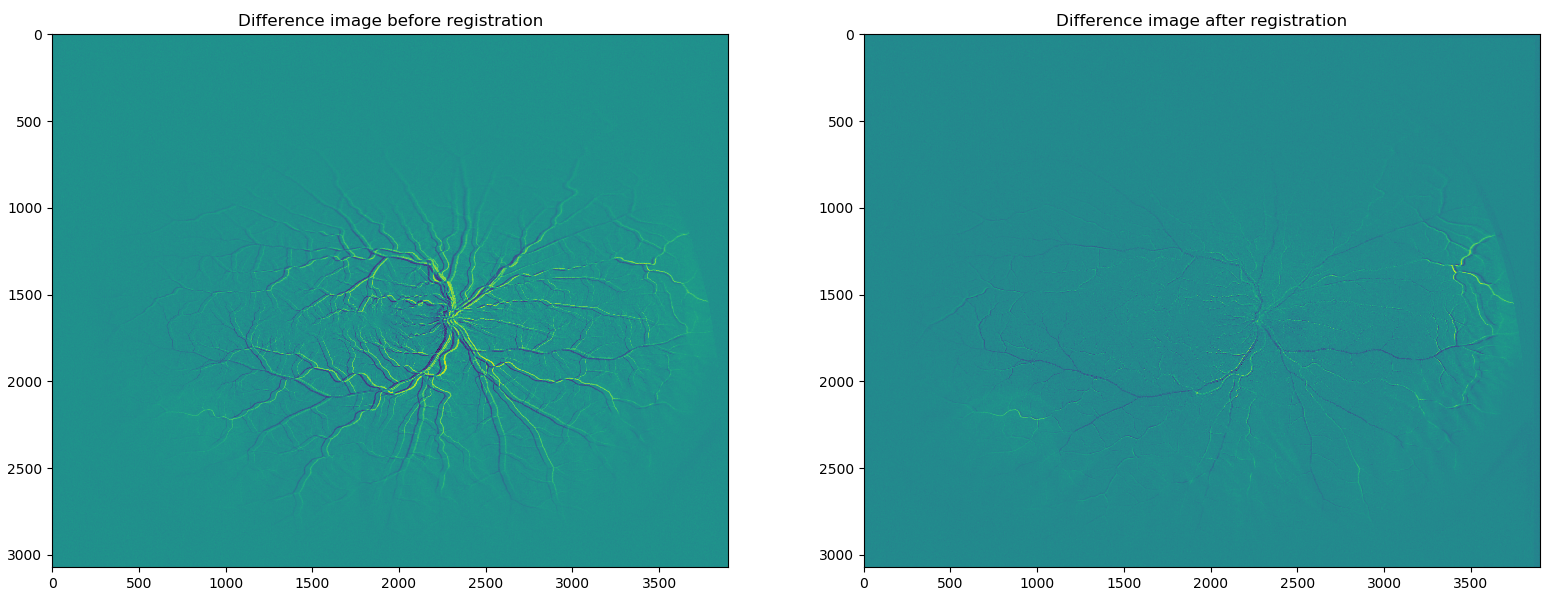
\includegraphics[width=0.8\textwidth]{figure/registration.png}
    \caption{The demonstration of image registration based on MINE loss.}
\label{fig_bay}
\end{figure*}

% registration.png

\section*{Question 2}
\label{sec_q2}
We extend the function \textbf{MatrixExp} into a class, in order to implement our own back propagation rule.
The source code is shown as follows: 
\begin{lstlisting}
class MatrixExp(Function):

    @staticmethod
    def forward(ctx, C):
        A = torch.eye(3).to(device)

        H = A
        for i in torch.arange(1, `\textbf{100}`):
            A = torch.mm(A/i, C)
            H = H + A

        ctx.save_for_backward(H)
        return H

    @staticmethod
    def backward(ctx, grad_output):
        result, = ctx.saved_tensors

        return torch.mm(grad_output, result)
\end{lstlisting}
You can also check the file ``\textbf{question2.py}'' for more details.
The program is running much faster than the old one.
In addition, the iteration number of Taylor series is increased to 100 to demonstrate that our own backpropagation rule makes the program faster.
We proposed a comparison between the program with class MatrixExp and the old program to demonstrate the efficiency,
which is shown as \reffig{fig2}. As we can see, the old program takes 112 seconds but the program with our own backpropagation only takes 46 seconds.

\begin{figure*}[htbp]	% FIGURE: figure/fig1 
\centering
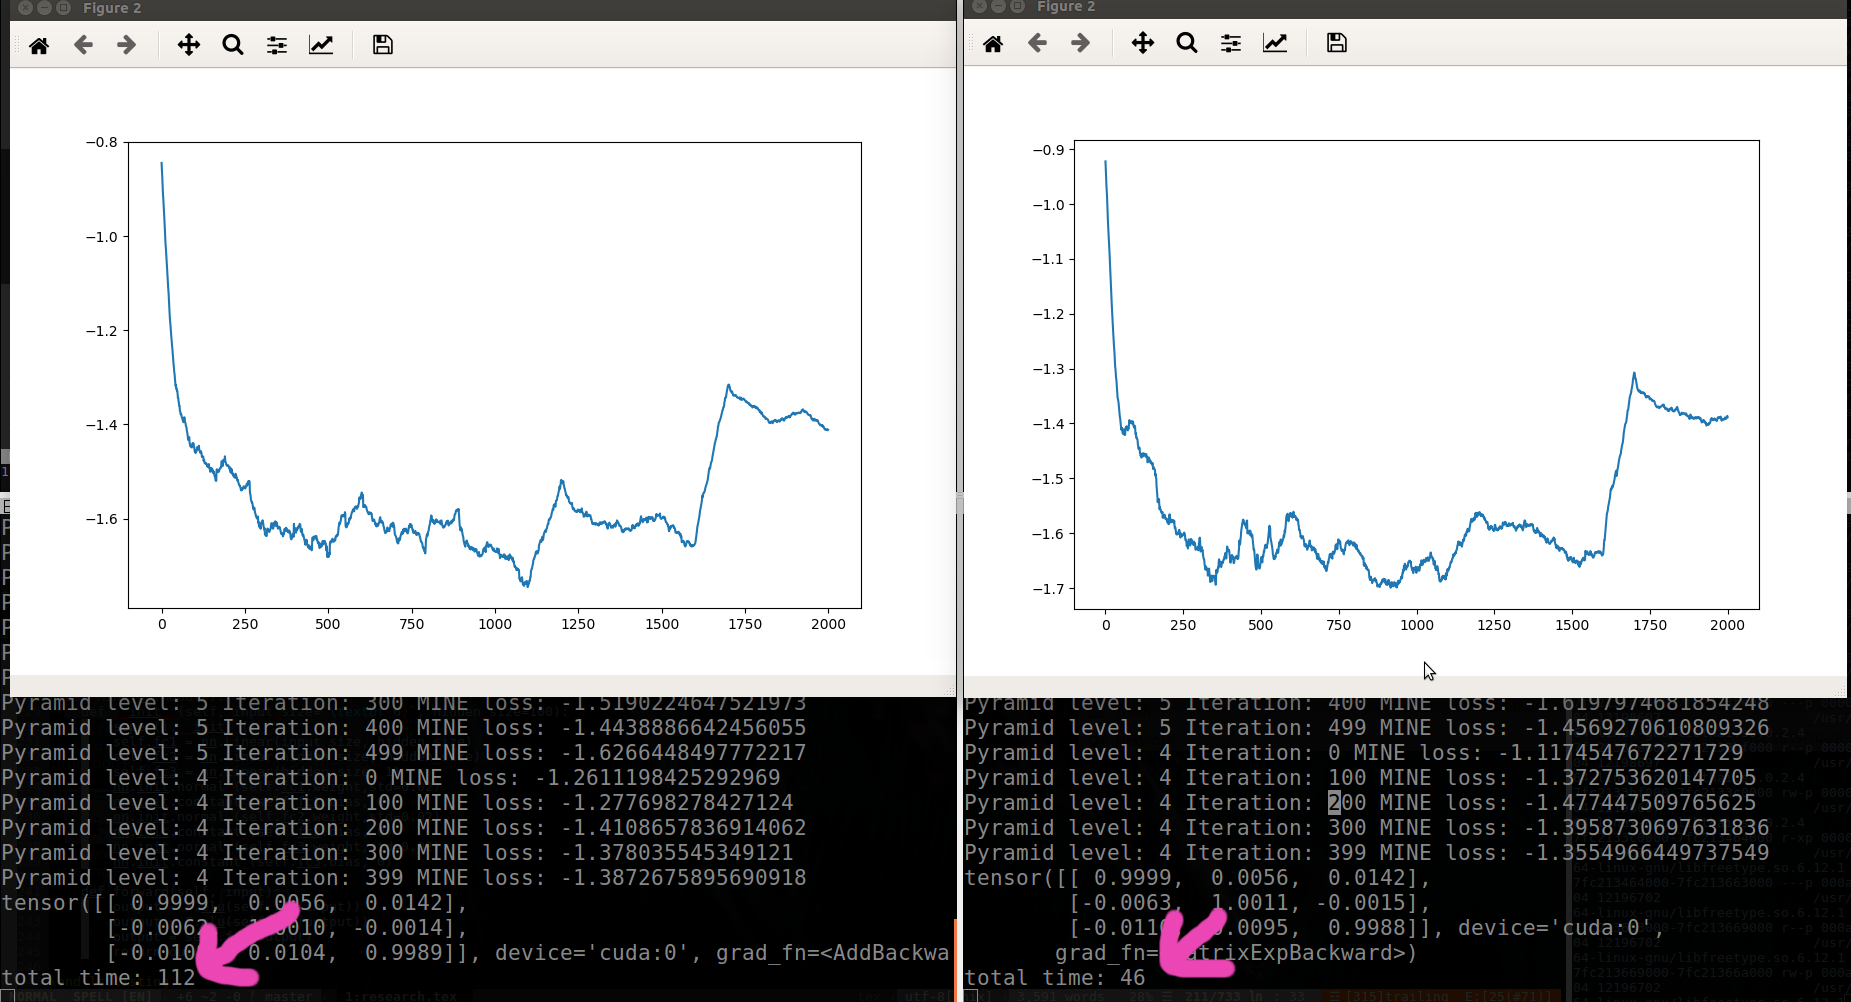
\includegraphics[width=0.99\textwidth]{figure/matrixexp.png}
    \caption{The comparison between problem with our own derivative rule and the original one. The running time of program with our own backpropagation rule is shown in the right part.}
\label{fig2}
\end{figure*} 
\   \\\\\\\\\\







\section*{Question 3}
\label{sec_q3}
To extend our program to color image,
the channel of MINE loss is increased to 6.
The \textbf{sample\_batch} function is modified for data with 6 channel,
and the function \textbf{PerspectiveTransform} is also extended to for transforming color image.
Please check ``\textbf{question3.py}'' for more details.
The source codes of these key functions are shown as follows:
\begin{lstlisting}
class Mine(nn.Module):
    def __init__(self, input_size=`\textbf{6}`, hidden_size=100):
        super().__init__()
        self.fc1 = nn.Linear(input_size, hidden_size)
        self.fc2 = nn.Linear(hidden_size, hidden_size)
        self.fc3 = nn.Linear(hidden_size, 1)
        nn.init.normal_(self.fc1.weight,std=0.02)
        nn.init.constant_(self.fc1.bias, 0)
        nn.init.normal_(self.fc2.weight,std=0.02)
        nn.init.constant_(self.fc2.bias, 0)
        nn.init.normal_(self.fc3.weight,std=0.02)
        nn.init.constant_(self.fc3.bias, 0)

    def forward(self, input):
        output = F.elu(self.fc1(input))
        output = F.elu(self.fc2(output))
        output = self.fc3(output)
        return output

\end{lstlisting}

\begin{lstlisting}
def sample_batch(data, batch_size=100, sample_mode='joint'):
    if sample_mode == 'joint':
        index = np.random.choice(range(data.shape[0]), size=batch_size, replace=False)
        batch = data[index]

    else:
        joint_index = np.random.choice(range(data.shape[0]), size=batch_size, replace=False)
        marginal_index = np.random.choice(range(data.shape[0]), size=batch_size, replace=False)

        `\textbf{batch\_joint = data[joint\_index, 0:3]}`
        `\textbf{batch\_marginal = data[marginal\_index, 3:6]}`

        `\textbf{batch = torch.cat( (batch\_joint, batch\_marginal) , 1)}`
    return batch
\end{lstlisting}


\begin{lstlisting}
def PerspectiveTransform(I, H, xv, yv):

    height, width, byte = I.shape

    xvt = (xv*H[0,0]+yv*H[0,1]+H[0,2])/(xv*H[2,0]+yv*H[2,1]+H[2,2])
    yvt = (xv*H[1,0]+yv*H[1,1]+H[1,2])/(xv*H[2,0]+yv*H[2,1]+H[2,2])

    `\textbf{J0 = F.grid\_sample(I[:, :, 0].view(1,1,height,width),torch.stack([xvt,yvt],2).unsqueeze(0)).squeeze()}`
    `\textbf{J1 = F.grid\_sample(I[:, :, 1].view(1,1,height,width),torch.stack([xvt,yvt],2).unsqueeze(0)).squeeze()}`
    `\textbf{J2 = F.grid\_sample(I[:, :, 2].view(1,1,height,width),torch.stack([xvt,yvt],2).unsqueeze(0)).squeeze()}`

    `\textbf{J0 = J0.unsqueeze(2)}`
    `\textbf{J1 = J1.unsqueeze(2)}`
    `\textbf{J2 = J2.unsqueeze(2)}`

    `\textbf{J = torch.cat((J0, J1, J2), 2)}`

    return J
\end{lstlisting}

\begin{figure*}[htbp]	% FIGURE: figure/fig1 
\centering
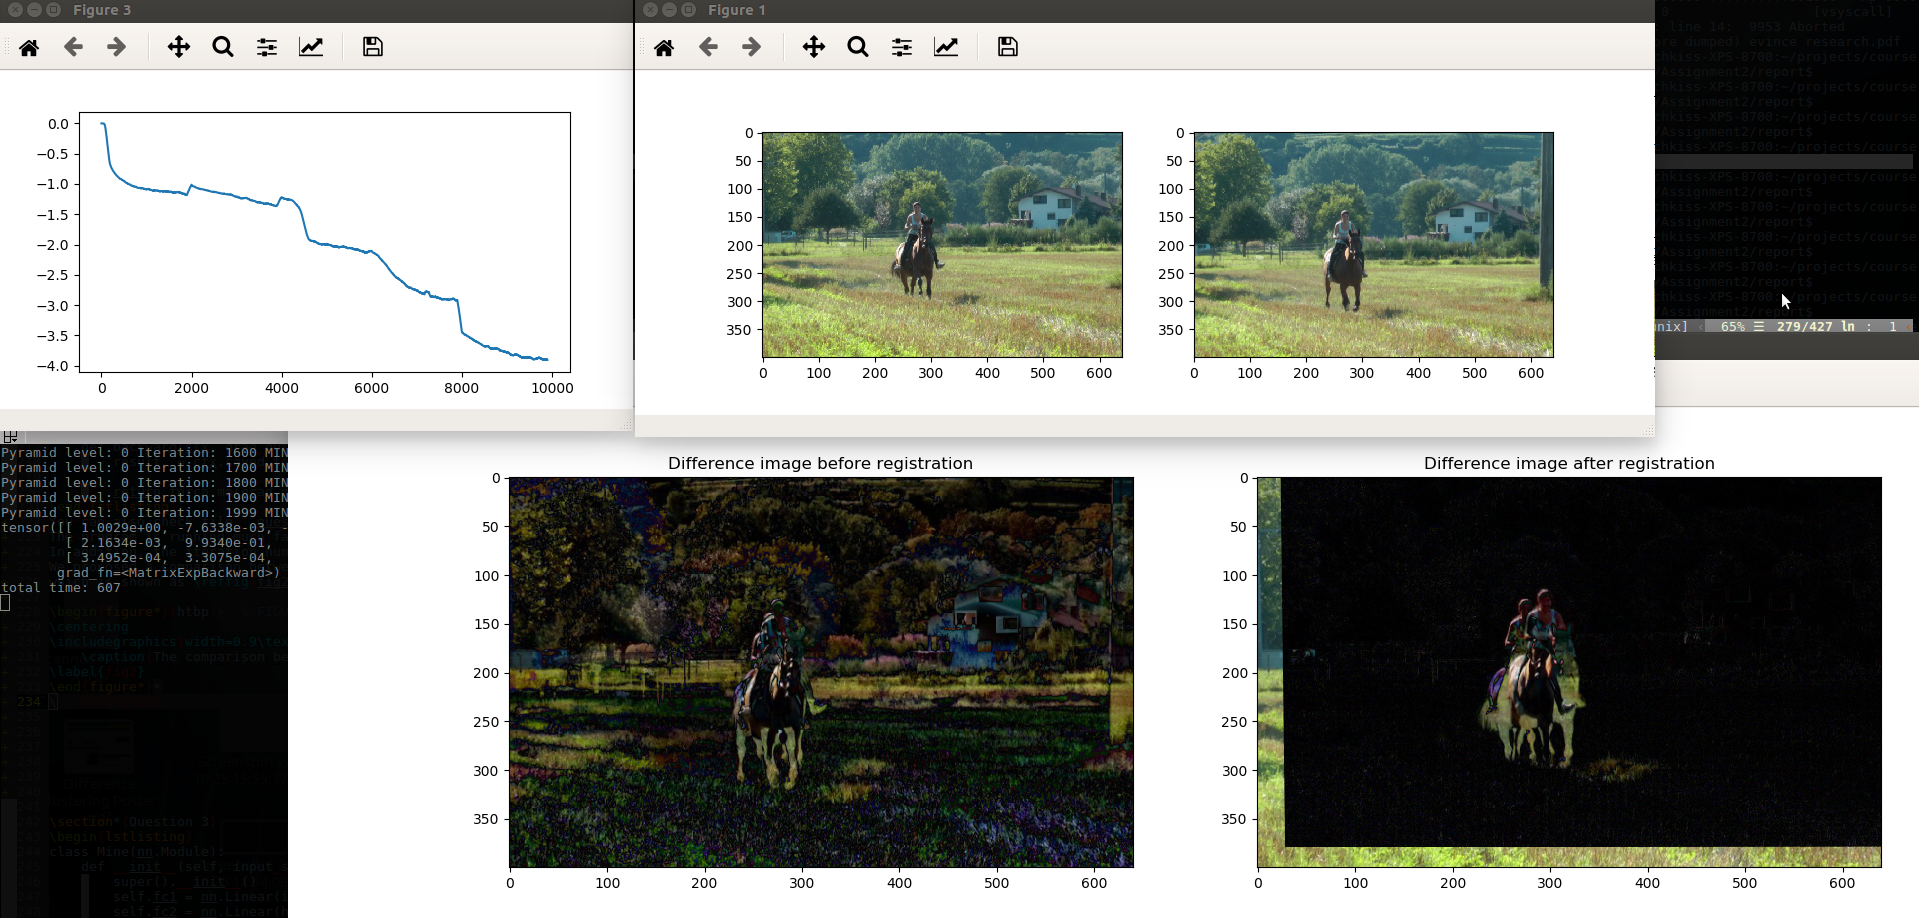
\includegraphics[width=0.99\textwidth]{figure/registration_color.png}
    \caption{The demonstration of color image registration based on MINE loss.}
\label{fig_bay}
\end{figure*}


\newpage




% \section*{Abstract}
% % 以前方法都是用
% Previous approaches to background subtraction typically proposed artificial model to approximate the distribution of pixels' observations.
% % 为什么distribution 可以用
% In this proposal, we focus on learning the distribution of observations automatically instead of devising sophisticated model.
% %
% In particular,
% the deep learning network is naturally selected to learn the distribution,
% due to it is excellent learning ability.
% %
% Moreover,
% distribution itself has wide range of applications as well.
% %
% Therefore, the distribution learning can not only be used in the background subtraction but also in many other fields.
% %
% Hence,
% just like the hierarchical features learned by deep learning network,
% we assume that there is high level representation of distribution which should work better than all these existed statistic techniques related to distribution,
% and we named this level representation as "Deep Distribution", which is the final target of this proposal.
% %
% 

% 以前distribution的确定是什么

% 你打算怎么做

% 具体怎么做

% 可以做成个什么样子


\section*{Question 4}
\label{sec_q4}
\begin{equation}
J(f)=\int_{}^{}f(x,z)P_{X,Z}(x,z)dxdz - ln(\int_{}^{}e^{f(x,z)}P_X(x)P_Z(z)dxdz)
\end{equation}

\begin{equation}
Let \quad f(x,z) = \bar{f}(x,z)+\varepsilon\eta, \quad \eta=g(x,z)
\end{equation}

\begin{equation}
\begin{split}
G(\varepsilon) & = J(\bar{f}(x,z)+\varepsilon \eta ) \\
    & =\int_{}^{} ( \bar{f}(x,z)+\varepsilon \eta ) P_{X,Z}(x,z)dxdz - ln(\int_{}^{}e^{\bar{f}(x,z)+\varepsilon \eta}P_X(x)P_Z(z)dxdz)
\end{split}
\end{equation}


\begin{equation}
   \begin{split}
       \label{eq_g}
   \frac{d G(\varepsilon)}{d \varepsilon}& = 
  \frac{d \left( \int_{}^{} ( \bar{f}(x,z)+\varepsilon \eta ) P_{X,Z}(x,z)dxdz - ln(\int_{}^{}e^{\bar{f}(x,z)+\varepsilon \eta}P_X(x)P_Z(z)dxdz) \right) }{d \varepsilon} \\
 & = \frac{d \left( \int_{}^{} ( \bar{f}(x,z)+\varepsilon \eta ) P_{X,Z}(x,z)dxdz \right) }{d \varepsilon} -  \frac{ d \left( ln(\int_{}^{}e^{\bar{f}(x,z)+\varepsilon \eta}P_X(x)P_Z(z)dxdz) \right)}{d \varepsilon}
 \end{split}
\end{equation}

According to the Leibniz integral rule:
\begin{equation}
\frac{d}{dx}\left( \int_{a}^{b}f(x,t)dt \right) = \int_{a}^{b}\frac{\partial}{\partial x}f(x,t)dt
\end{equation}

we get:
\begin{equation}
    \begin{split}
          & \frac{d \left( \int_{}^{} ( \bar{f}(x,z)+\varepsilon \eta ) P_{X,Z}(x,z)dxdz \right) }{d \varepsilon} \\
        = & \int_{}^{} \frac{\partial \left( ( \bar{f}(x,z)+\varepsilon \eta ) P_{X,Z}(x,z)dxdz \right)}{\partial \varepsilon} \\ 
        = & \int_{}^{} \frac{\partial \left( \bar{f}(x,z) P_{X,Z}(x,z)dxdz \right)}{\partial \varepsilon} + \int_{}^{} \frac{\partial \left( ( \varepsilon \eta ) P_{X,Z}(x,z)dxdz \right)}{\partial \varepsilon} \\ 
        = & 0 + \int_{}^{} \frac{\partial (\varepsilon \eta)}{\partial \varepsilon}    P_{X,Z}(x,z)dxdz  \\ 
        = & \int_{}^{}    \eta  P_{X,Z}(x,z)dxdz
    \end{split}
\end{equation}

\begin{equation}
    \begin{split}
            & \frac{ d \left( ln(\int_{}^{}e^{\bar{f}(x,z)+\varepsilon \eta}P_X(x)P_Z(z)dxdz) \right)}{d \varepsilon} \\ 
        = & \frac{1}{\int_{}^{}e^{\bar{f}(x,z)+\varepsilon \eta}P_X(x)P_Z(z)dxdz} \cdot  \frac{ d \left( \int_{}^{}e^{\bar{f}(x,z)+\varepsilon \eta}P_X(x)P_Z(z)dxdz \right)}{d \varepsilon} \\ 
        = & \frac{1}{\int_{}^{}e^{\bar{f}(x,z)+\varepsilon \eta}P_X(x)P_Z(z)dxdz} \cdot  \int_{}^{} \frac{ \partial \left( e^{\bar{f}(x,z)+\varepsilon \eta}P_X(x)P_Z(z)dxdz \right) }{\partial \varepsilon} \\ 
        = & \frac{1}{\int_{}^{}e^{\bar{f}(x,z)+\varepsilon \eta}P_X(x)P_Z(z)dxdz} \cdot  \int_{}^{} \frac{ \partial  e^{\bar{f}(x,z)+\varepsilon \eta}   }{\partial \varepsilon}P_X(x)P_Z(z)dxdz \\ 
        = & \frac{1}{\int_{}^{}e^{\bar{f}(x,z)+\varepsilon \eta}P_X(x)P_Z(z)dxdz} \cdot  \int_{}^{} e^{\bar{f}(x,z)+\varepsilon \eta} \frac{ \partial  (\bar{f}(x,z)+\varepsilon \eta)   }{\partial \varepsilon}P_X(x)P_Z(z)dxdz \\ 
        = & \frac{1}{\int_{}^{}e^{\bar{f}(x,z)+\varepsilon \eta}P_X(x)P_Z(z)dxdz} \cdot  \int_{}^{} e^{\bar{f}(x,z)+\varepsilon \eta} \eta P_X(x)P_Z(z)dxdz \\
        = & \frac{\int_{}^{} e^{\bar{f}(x,z)+\varepsilon \eta} \eta P_X(x)P_Z(z)dxdz}{\int_{}^{}e^{\bar{f}(x,z)+\varepsilon \eta}P_X(x)P_Z(z)dxdz}
    \end{split}
\end{equation}

Then, the \refequ{eq_g} becomes:
\begin{equation}
    \begin{split}
        \frac{d G(\varepsilon)}{d \varepsilon} & = \frac{d \left( \int_{}^{} ( \bar{f}(x,z)+\varepsilon \eta ) P_{X,Z}(x,z)dxdz \right) }{d \varepsilon} -  \frac{ d \left( ln(\int_{}^{}e^{\bar{f}(x,z)+\varepsilon \eta}P_X(x)P_Z(z)dxdz) \right)}{d \varepsilon} \\
        & = \int_{}^{}    \eta  P_{X,Z}(x,z)dxdz  -  \frac{\int_{}^{} e^{\bar{f}(x,z)+\varepsilon \eta} \eta P_X(x)P_Z(z)dxdz}{\int_{}^{}e^{\bar{f}(x,z)+\varepsilon \eta}P_X(x)P_Z(z)dxdz}
    \end{split}
\end{equation}
In order to achieve the maximum value, we need $ \lim \limits_{\varepsilon \to 0} \frac{dG(\varepsilon)}{d \varepsilon} = 0  $. Then we get:

\begin{equation}
    \label{eq_res1}
    \begin{split}
        & \lim_{\varepsilon \to 0} \frac{d G(\varepsilon)}{d \varepsilon}  = \lim_{\varepsilon \to 0} \left( \int_{}^{}    \eta  P_{X,Z}(x,z)dxdz  -  \frac{\int_{}^{} e^{\bar{f}(x,z)+\varepsilon \eta} \eta P_X(x)P_Z(z)dxdz}{\int_{}^{}e^{\bar{f}(x,z)+\varepsilon \eta}P_X(x)P_Z(z)dxdz} \right) = 0 \\
        & \Rightarrow \int_{}^{}    \eta  P_{X,Z}(x,z)dxdz  -  \lim_{\varepsilon \to 0} \left(\frac{\int_{}^{} e^{\bar{f}(x,z)+\varepsilon \eta} \eta P_X(x)P_Z(z)dxdz}{\int_{}^{}e^{\bar{f}(x,z)+\varepsilon \eta}P_X(x)P_Z(z)dxdz} \right) = 0 \\
        & \Rightarrow \int_{}^{}    \eta  P_{X,Z}(x,z)dxdz  =  \lim_{\varepsilon \to 0} \left(\frac{\int_{}^{} e^{\bar{f}(x,z)+\varepsilon \eta} \eta P_X(x)P_Z(z)dxdz}{\int_{}^{}e^{\bar{f}(x,z)+\varepsilon \eta}P_X(x)P_Z(z)dxdz} \right) \\
        & \Rightarrow \int_{}^{}    \eta  P_{X,Z}(x,z)dxdz  =  \frac{\int_{}^{} e^{\bar{f}(x,z)+0\cdot \eta} \eta P_X(x)P_Z(z)dxdz}{\int_{}^{}e^{\bar{f}(x,z)+0 \cdot \eta}P_X(x)P_Z(z)dxdz} \\
        & \Rightarrow \int_{}^{}    \eta  P_{X,Z}(x,z)dxdz  =  \frac{\int_{}^{} e^{\bar{f}(x,z)} \eta P_X(x)P_Z(z)dxdz}{\int_{}^{}e^{\bar{f}(x,z)}P_X(x)P_Z(z)dxdz} \\
        & \Rightarrow \int_{}^{}    \eta  \left( P_{X,Z}(x,z) \right) dxdz  =\int_{}^{}    \eta \left( \frac{ e^{\bar{f}(x,z)}  P_X(x)P_Z(z)}{\int_{}^{}e^{\bar{f}(x,z)}P_X(x)P_Z(z)dxdz}\right) dxdz \quad \because \eta \neq 0  \\ 
        & \Rightarrow  \textcolor{red}{ P_{X,Z}(x,z) = \frac{ e^{\bar{f}(x,z)}  P_X(x)P_Z(z)}{\int_{}^{}e^{\bar{f}(x,z)}P_X(x)P_Z(z)dxdz} }
    \end{split}
\end{equation}

With the \refequ{eq_res1}, we have:
\begin{equation}
    \begin{split}
        & P_{X,Z}(x,z) = \frac{ e^{\bar{f}(x,z)}  P_X(x)P_Z(z)}{\int_{}^{}e^{\bar{f}(x,z)}P_X(x)P_Z(z)dxdz} \\
        \Rightarrow & e^{\bar{f}(x,z)} = \frac{P_{X,Z}(x,z) \int_{}^{}e^{\bar{f}(x,z)}P_X(x)P_Z(z)dxdz }{P_X(x)P_Z(z)} \\
        \Rightarrow & \bar{f}(x,z) = ln \left( \frac{P_{X,Z}(x,z) \int_{}^{}e^{\bar{f}(x,z)}P_X(x)P_Z(z)dxdz }{P_X(x)P_Z(z)} \right) \\
        \Rightarrow & \bar{f}(x,z) = ln \left( \frac{P_{X,Z}(x,z) \int_{}^{}e^{\bar{f}(x,z)}P_X(x)P_Z(z)dxdz }{P_X(x)P_Z(z)} \right) \\
        \Rightarrow & \bar{f}(x,z) = ln \left( \frac{P_{X,Z}(x,z) }{P_X(x)P_Z(z)} \right) + ln\left(\int_{}^{}e^{\bar{f}(x,z)}P_X(x)P_Z(z)dxdz  \right)
    \end{split}
\end{equation}

Then, we plug $\bar{f}(x,z)$ into $J(f)$:
\begin{equation}
    \begin{split}
        J(\bar{f}(x,z))  = & \int_{}^{}\bar{f}(x,z)P_{X,Z}(x,z)dxdz - ln\left(  \int_{}^{} e^{\bar{f}(x,z)}P_X(x)P_Z(z)dxdz \right) \\
        = & \int_{}^{}\left[ ln \left( \frac{P_{X,Z}(x,z) }{P_X(x)P_Z(z)} \right) + ln\left(\int_{}^{}e^{ \bar{f}(x,z) }P_X(x)P_Z(z)dxdz  \right)  \right] P_{X,Z}(x,z)dxdz \\
        & \quad - ln\left(  \int_{}^{} e^{\bar{f}(x,z)}P_X(x)P_Z(z)dxdz \right) \\
        = & \int_{}^{} ln \left( \frac{P_{X,Z}(x,z) }{P_X(x)P_Z(z)} \right)P_{X,Z}(x,z)dxdz + \int_{}^{} ln\left(\int_{}^{}e^{ \bar{f}(x,z) }P_X(x)P_Z(z)dxdz  \right) P_{X,Z}(x,z)dxdz  \\
        & \quad - ln\left(  \int_{}^{} e^{\bar{f}(x,z)}P_X(x)P_Z(z)dxdz \right) \\
        = & \int_{}^{} ln \left( \frac{P_{X,Z}(x,z) }{P_X(x)P_Z(z)} \right)P_{X,Z}(x,z)dxdz + ln\left(\int_{}^{}e^{ \bar{f}(x,z) }P_X(x)P_Z(z)dxdz  \right) \int_{}^{} P_{X,Z}(x,z)dxdz  \\
        & \quad - ln\left(  \int_{}^{} e^{\bar{f}(x,z)}P_X(x)P_Z(z)dxdz \right) \quad \because \int_{}^{}   P_{X,Z}(x,z)dxdz = 1 \\
        = & \int_{}^{} ln \left( \frac{P_{X,Z}(x,z) }{P_X(x)P_Z(z)} \right)P_{X,Z}(x,z)dxdz + ln\left(\int_{}^{}e^{ \bar{f}(x,z) }P_X(x)P_Z(z)dxdz  \right) \cdot 1 \\
        & \quad - ln\left(  \int_{}^{} e^{\bar{f}(x,z)}P_X(x)P_Z(z)dxdz \right) \\
        = & \int_{}^{} ln \left( \frac{P_{X,Z}(x,z) }{P_X(x)P_Z(z)} \right)P_{X,Z}(x,z)dxdz  \\
        \Rightarrow \textcolor{red}{  J(\bar{f}(x,z)) = } & \textcolor{red}{ \int_{}^{} ln \left( \frac{P_{X,Z}(x,z) }{P_X(x)P_Z(z)} \right)P_{X,Z}(x,z)dxdz}
    \end{split}
\end{equation}






\end{document}
